\documentclass[10pt,a4paper]{beamer}
\usepackage[utf8]{inputenc}
\usepackage[francais]{babel}
\usepackage[T1]{fontenc}
\usepackage{amsmath}

\usepackage{amsfonts}
\usepackage{amssymb}

\usetheme[secheader]{Boadilla}


\usepackage[usenames,dvipsnames]{pstricks}


\title[Présentation Petit Dej]{Extension de la PGD à des problèmes de dynamique non-linéaires}
\author[Pierre NARGIL]{Pierre NARGIL\\Encadrants : 
\large{\\François LOUF\\Pierre-Alain BOUCARD} }
\institute{LMT Cachan}
\date{Mardi 15 Juillet 2014}


\begin{document}

\begin{frame}
	\titlepage
\end{frame}

\begin{frame}
	\begin{itemize}
		\item TDG dans tous les cas : adaptation manquante de TDG au multiplicateurs de Lagrange.
		\item Autres codes
		\item Modification du programme pour utiliser des structures
		\item Utilisation de TDG avec la PGD
		\item Tentative de modification de la pénalisation pour permettre plus ou moins de discontinuité
		\item Solution Exactes
		\item Notes
	\end{itemize}
\end{frame}

\begin{frame}{Autres Codes}
	\begin{itemize}
		\item Le code de Pierre-Éric
			\begin{itemize}
				\item Généralisation
				\item Obscur
			\end{itemize}
		\item Le projet commun
			\begin{itemize}
				\item Départ de Hugo. 
			\end{itemize}
	\end{itemize}
\end{frame}

\begin{frame}{Utilisation des structures}
	\begin{itemize}
		\item Rendre le programme plus lisible
		\item Autoriser une forme de polymorphisme
			\begin{itemize}
				\item Création de nouveaux objets pour utiliser les fonctions discontinues de la TDG
				sans devoir refaire ou dédoubler chaque fonction du programme.
				\item Possibilité de classes / polymorphisme sous castem ?
			\end{itemize}
	\end{itemize}
\end{frame}

\begin{frame}{Utilisation de TDG avec la PGD}
	\begin{itemize}
		\item Équations calculées
		\item Programmation / Résultats
			\begin{itemize}
				\item Un seul mode trouvé (mis à part une fois)
				\item stagnation quasi parfaite
			\end{itemize}
	\end{itemize}
\end{frame}

\begin{frame}{Modification de la pénalisation}
	\begin{itemize}
		\item Pourquoi : 
			\begin{itemize}
				\item Constat : discontinuités très faibles
				\item Voir l'influence sur convergence et la qualité de la solution
			\end{itemize}
		\item Comment : Changer le coefficient multipliant le saut de U
		\item 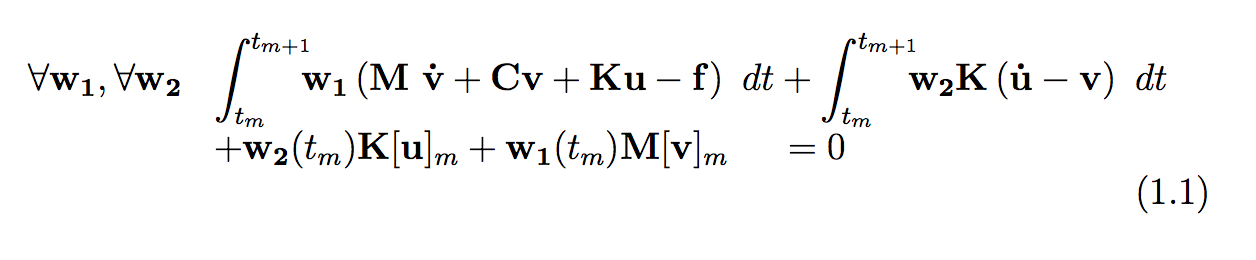
\includegraphics[width=0.8\linewidth]{TDG_1-1.png}
		\item Programmation - Résultat
			\begin{itemize}
				\item Équations obtenues par le programme Maple
				\item Résolution divergente
			\end{itemize}
	\end{itemize}
\end{frame}

\begin{frame}{Solution exactes}
	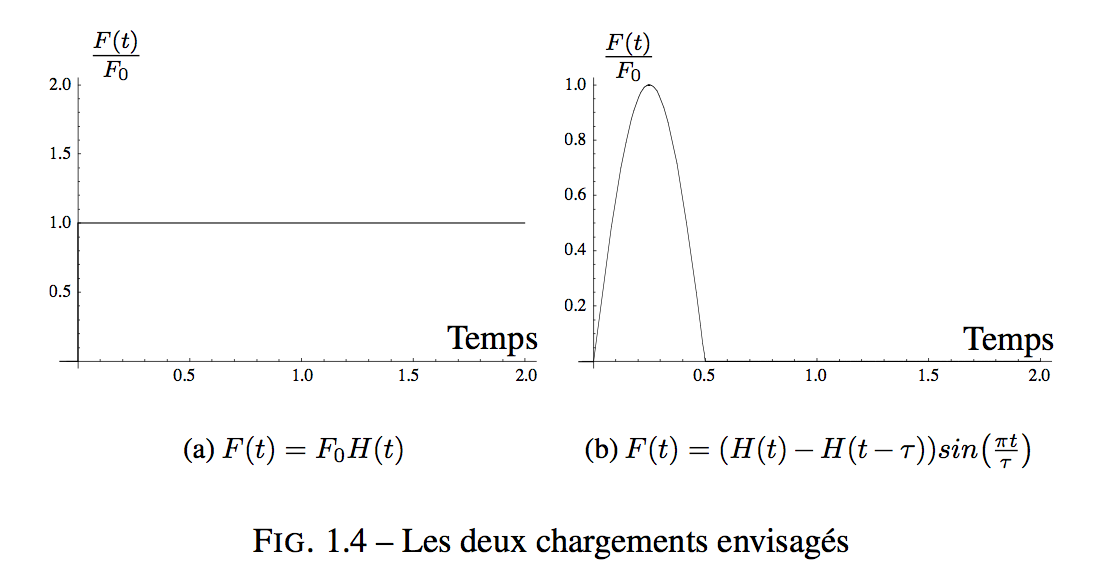
\includegraphics[width=0.8\linewidth]{Sinus.png}
	\begin{itemize}
		\item Le sinus verse : remplacer sin(•) par (1 + cos(•) )
		\item Résolution de l'équation différentielles plus complexe : on ne peut plus factoriser par $\alpha$
		\item Les bugs Maple et les sommes Matlab et le moins indispensable
	\end{itemize}
\end{frame}

\begin{frame}{Notes}
	\begin{itemize}
		\item Forme de rapport d’erreur
		\item Les solution en modèle réduit semblent être plus proche de la solution complète 
		\item Communication : Vendredi
	\end{itemize}
\end{frame}

\end{document}
